\section{GtkDrawingArea and Cairo}\label{gtkdrawingarea-and-cairo}

If you want to draw shapes or paint images dynamically on the screen,
use the GtkDrawingArea widget.

GtkDrawingArea provides a cairo drawing context. You can draw images
with cairo library functions. This section describes:

\begin{enumerate}
\def\labelenumi{\arabic{enumi}.}
\tightlist
\item
  Cairo, but briefly
\item
  GtkDrawingArea, with a very simple example.
\end{enumerate}

\subsection{Cairo}\label{cairo}

Cairo is a drawing library for two dimensional graphics. There are a lot
of documents on \href{https://www.cairographics.org/}{Cairo's website}.
If you aren't familiar with Cairo, it is worth reading the
\href{https://www.cairographics.org/tutorial/}{tutorial}.

The following is an introduction to the Cairo library. First, you need
to know surfaces, sources, masks, destinations, cairo context and
transformations.

\begin{itemize}
\tightlist
\item
  A surface represents an image. It is like a canvas. We can draw shapes
  and images with different colors on surfaces.
\item
  The source pattern, or simply source, is like paint, which will be
  transferred to destination surface by cairo functions.
\item
  The mask describes the area to be used in the copy;
\item
  The destination is a target surface;
\item
  The cairo context manages the transfer from source to destination,
  through mask with its functions; For example,
  \passthrough{\lstinline!cairo\_stroke!} is a function to draw a path
  to the destination by the transfer.
\item
  A transformation can be applied before the transfer completes. The
  transformation which is applied is called affine, which is a
  mathematical term meaning transofrmations that preserve straight
  lines. Scaling, rotating, reflecting, shearing and translating are
  examples of affine transformations. They are mathematically
  represented by matrix multiplication and vector addition. In this
  section we don't use it, instead we will only use the identity
  transformation. This means that the coordinates in the source and mask
  are the same as the coordinates in destination.
\end{itemize}

\begin{figure}
\centering
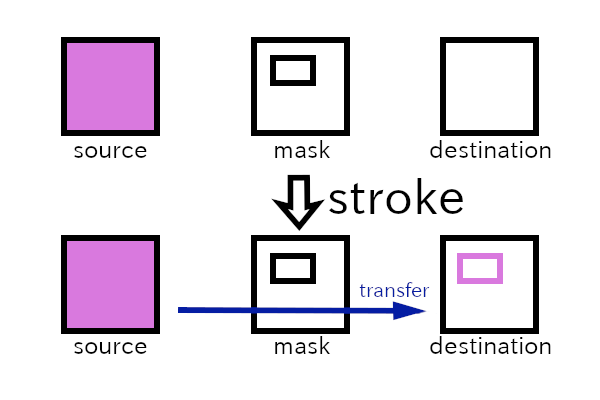
\includegraphics[width=9cm,height=6cm]{../image/cairo.png}
\caption{Stroke a rectangle}
\end{figure}

The instruction is as follows:

\begin{enumerate}
\def\labelenumi{\arabic{enumi}.}
\tightlist
\item
  Create a surface. This will be the destination.
\item
  Create a cairo context with the surface, the surface will be the
  destination of the context.
\item
  Create a source pattern within the context.
\item
  Create paths, which are lines, rectangles, arcs, texts or more
  complicated shapes in the mask.
\item
  Use a drawing operator such as \passthrough{\lstinline!cairo\_stroke!}
  to transfer the paint in the source to the destination.
\item
  Save the destination surface to a file if necessary.
\end{enumerate}

Here's a simple example program that draws a small square and saves it
as a png file. The path of the file is
\passthrough{\lstinline!src/misc/cairo.c!}.

\begin{lstlisting}[language=C, numbers=left]
#include <cairo.h>

int
main (int argc, char **argv)
{
  cairo_surface_t *surface;
  cairo_t *cr;
  int width = 100;
  int height = 100;
  int square_size = 40.0;

  /* Create surface and cairo */
  surface = cairo_image_surface_create (CAIRO_FORMAT_RGB24, width, height);
  cr = cairo_create (surface);

  /* Drawing starts here. */
  /* Paint the background white */
  cairo_set_source_rgb (cr, 1.0, 1.0, 1.0);
  cairo_paint (cr);
  /* Draw a black rectangle */
  cairo_set_source_rgb (cr, 0.0, 0.0, 0.0);
  cairo_set_line_width (cr, 2.0);
  cairo_rectangle (cr,
                   width/2.0 - square_size/2,
                   height/2.0 - square_size/2,
                   square_size,
                   square_size);
  cairo_stroke (cr);

  /* Write the surface to a png file and clean up cairo and surface. */
  cairo_surface_write_to_png (surface, "rectangle.png");
  cairo_destroy (cr);
  cairo_surface_destroy (surface);

  return 0;
}
\end{lstlisting}

\begin{itemize}
\tightlist
\item
  1: Includes the header file of Cairo.
\item
  6: \passthrough{\lstinline!cairo\_surface\_t!} is the type of a
  surface.
\item
  7: \passthrough{\lstinline!cairo\_t!} is the type of a cairo context.
\item
  8-10: \passthrough{\lstinline!width!} and
  \passthrough{\lstinline!height!} are the size of
  \passthrough{\lstinline!surface!}.
  \passthrough{\lstinline!square\_size!} is the size of a square to be
  drawn on the surface.
\item
  13: \passthrough{\lstinline!cairo\_image\_surface\_create!} creates an
  image surface. \passthrough{\lstinline!CAIRO\_FORMAT\_RGB24!} is a
  constant which means that each pixel has red, green and blue data, and
  each data point is an 8 bits number (for 24 bits in total). Modern
  displays have this type of color depth. Width and height are in pixels
  and given as integers.
\item
  14: Creates cairo context. The surface given as an argument will be
  the destination of the context.
\item
  18: \passthrough{\lstinline!cairo\_set\_source\_rgb!} creates a source
  pattern, which is a solid white paint. The second to fourth arguments
  are red, green and blue color values respectively, and they are of
  type float. The values are between zero (0.0) and one (1.0). Black is
  (0.0,0.0,0.0) and white is (1.0,1.0,1.0).
\item
  19: \passthrough{\lstinline!cairo\_paint!} copies everywhere in the
  source to destination. The destination is filled with white pixels
  with this command.
\item
  21: Sets the source color to black.
\item
  22: \passthrough{\lstinline!cairo\_set\_line\_width!} sets the width
  of lines. In this case, the line width is set to be two pixels and
  will end up that same size. (It is because the transformation is
  identity. If the transformation isn't identity, for example scaling
  with the factor three, the actual width in destination will be six
  (2x3=6) pixels.)
\item
  23: Draws a rectangle (square) on the mask. The square is located at
  the center.
\item
  24: \passthrough{\lstinline!cairo\_stroke!} transfers the source to
  destination through the rectangle in the mask.
\item
  31: Outputs the image to a png file
  \passthrough{\lstinline!rectangle.png!}.
\item
  32: Destroys the context. At the same time the source is destroyed.
\item
  33: Destroys the surface.
\end{itemize}

To compile this, change your current directory to
\passthrough{\lstinline!src/misc!} and type the following.

\begin{lstlisting}
$ gcc `pkg-config --cflags cairo` cairo.c `pkg-config --libs cairo`
\end{lstlisting}

s 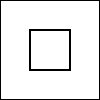
\includegraphics{../image/rectangle.png}

See the \href{https://www.cairographics.org/}{Cairo's website} for
further information.

\subsection{GtkDrawingArea}\label{gtkdrawingarea}

The following is a very simple example.

\begin{lstlisting}[language=C, numbers=left]
#include <gtk/gtk.h>

static void
draw_function (GtkDrawingArea *area, cairo_t *cr, int width, int height, gpointer user_data) {
  int square_size = 40.0;

  cairo_set_source_rgb (cr, 1.0, 1.0, 1.0); /* white */
  cairo_paint (cr);
  cairo_set_line_width (cr, 2.0);
  cairo_set_source_rgb (cr, 0.0, 0.0, 0.0); /* black */
  cairo_rectangle (cr,
                   width/2.0 - square_size/2,
                   height/2.0 - square_size/2,
                   square_size,
                   square_size);
  cairo_stroke (cr);
}

static void
app_activate (GApplication *app, gpointer user_data) {
  GtkWidget *win = gtk_application_window_new (GTK_APPLICATION (app));
  GtkWidget *area = gtk_drawing_area_new ();

  gtk_window_set_title (GTK_WINDOW (win), "da1");
  gtk_drawing_area_set_draw_func (GTK_DRAWING_AREA (area), draw_function, NULL, NULL);
  gtk_window_set_child (GTK_WINDOW (win), area);

  gtk_window_present (GTK_WINDOW (win));
}

#define APPLICATION_ID "com.github.ToshioCP.da1"

int
main (int argc, char **argv) {
  GtkApplication *app;
  int stat;

  app = gtk_application_new (APPLICATION_ID, G_APPLICATION_DEFAULT_FLAGS);
  g_signal_connect (app, "activate", G_CALLBACK (app_activate), NULL);
  stat =g_application_run (G_APPLICATION (app), argc, argv);
  g_object_unref (app);
  return stat;
}
\end{lstlisting}

The function \passthrough{\lstinline!main!} is almost same as before.
The two functions \passthrough{\lstinline!app\_activate!} and
\passthrough{\lstinline!draw\_function!} are important in this example.

\begin{itemize}
\tightlist
\item
  22: Creates a GtkDrawingArea instance.
\item
  25: Sets a drawing function of the widget. GtkDrawingArea widget uses
  the function \passthrough{\lstinline!draw\_function!} to draw the
  contents of itself whenever its necessary. For example, when a user
  drag a mouse pointer and resize a top-level window, GtkDrawingArea
  also changes the size. Then, the whole window needs to be redrawn. For
  the information of
  \passthrough{\lstinline!gtk\_drawing\_area\_set\_draw\_func!}, see
  \href{https://docs.gtk.org/gtk4/method.DrawingArea.set_draw_func.html}{Gtk
  API Reference -- gtk\_drawing\_area\_set\_draw\_func}.
\end{itemize}

The drawing function has five parameters.

\begin{lstlisting}[language=C]
void drawing_function (GtkDrawingArea *drawing_area, cairo_t *cr, int width, int height,
                       gpointer user_data);
\end{lstlisting}

The first parameter is the GtkDrawingArea widget. You can't change any
properties, for example \passthrough{\lstinline!content-width!} or
\passthrough{\lstinline!content-height!}, in this function. The second
parameter is a cairo context given by the widget. The destination
surface of the context is connected to the contents of the widget. What
you draw to this surface will appear in the widget on the screen. The
third and fourth parameters are the size of the destination surface.
Now, look at the program again.

\begin{itemize}
\tightlist
\item
  3-17: The drawing function.
\item
  7-8: Sets the source to be white and paint the destination white.
\item
  9: Sets the line width to be 2.
\item
  10: Sets the source to be black.
\item
  11-15: Adds a rectangle to the mask.
\item
  16: Draws the rectangle with black color to the destination.
\end{itemize}

The program is src/misc/da1.c. Compile and run it, then a window with a
black rectangle (square) appears. Try resizing the window. The square
always appears at the center of the window because the drawing function
is invoked each time the window is resized.

\begin{figure}
\centering
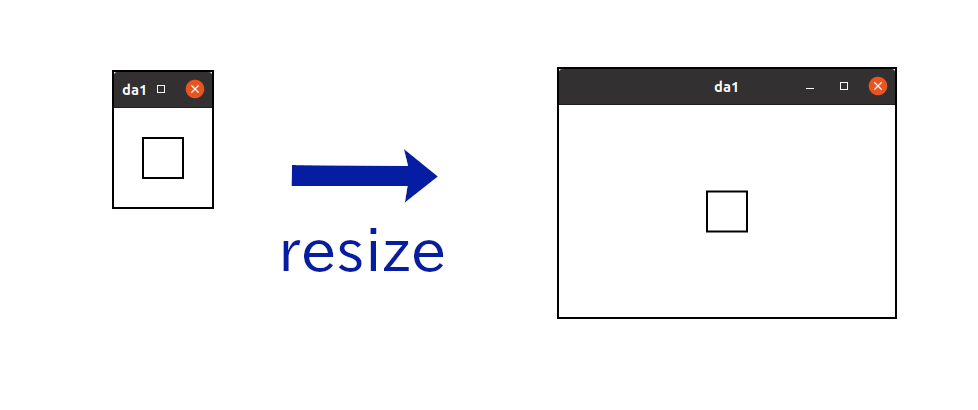
\includegraphics[width=8cm,height=3.4cm]{../image/da1.png}
\caption{Square in the window}
\end{figure}
